% ---------------------------------------------------------------------
%  The Turkey Problem revisited
%  Rewritten version.  To submit to an Elsevier journal, replace
%  \documentclass[11pt]{article} by \documentclass[preprint,12pt]{elsarticle}
%  and restore the \begin{frontmatter} block (commented at the end).
% ---------------------------------------------------------------------
\documentclass[11pt]{article}

\usepackage[T1]{fontenc}
\usepackage[utf8]{inputenc}
\usepackage{amsmath,amssymb}
\usepackage{graphicx}
\usepackage{booktabs}
\usepackage[margin=1in]{geometry}
\usepackage{siunitx}
\usepackage[hidelinks]{hyperref}

\sisetup{separate-uncertainty=true}
% non-SI units used in the sources (US roasting charts)
\DeclareSIUnit{\pound}{lb}
\DeclareSIUnit{\degreeFahrenheit}{\ensuremath{^{\circ}}F}

\newcommand{\Bi}{\mathit{Bi}}
\newcommand{\Fo}{\mathit{Fo}}

\title{\textbf{The turkey problem revisited:\\
what dimensional analysis can and cannot decide}}
\author{%
  l0d0v1c \quad pseudoLucV7\\[2pt]
  \small\url{https://github.com/l0d0v1c/TurkeyDimensional}}
\date{\today}

\begin{document}
\maketitle

\begin{abstract}
\noindent
A textbook exercise in dimensional analysis asks how long a \SI{10}{\pound}
turkey takes to roast given that a \SI{5}{\pound} turkey takes five hours.
Two things are wrong with it. First, its data are fictitious: published
roasting charts give roughly three hours for a \SI{10}{\pound} bird, not
five or eight. Second, the standard answer $t \propto m^{2/3}$ is presented
as \emph{the} consequence of dimensional analysis when it is in fact the
consequence of one modelling choice among several.
We show that enumerating dimensionally admissible monomials over an
over-specified variable set --- one that contains both the thermal
diffusivity $\alpha$ and its constituents $k$, $\rho$, $c$, and both the mass
$m$ and the length $l$ they determine --- generates sixteen formulae that
collapse to six, and that ten of those sixteen retain the absolute
temperature $T$ even though the governing equation is linear in
temperature and cannot contain it. Correctly posed, the problem yields a
single group, $\Fo = t\alpha/l^{2} = F(\Bi,\theta)$.
We then fit published roasting charts by weighted log--log regression
rather than by correlation coefficients, which we show are incapable of
discriminating between candidate exponents. The measured exponent is
$n = \num{0.54 \pm 0.02}$, excluding $n=1$ at $7.5\sigma$ and lying below
the isothermal-surface value $2/3$. A finite-Biot calculation reproduces
$n_{\text{eff}} = 0.54$--$0.60$ for realistic oven heat-transfer
coefficients, so the deviation is a consequence of the diffusive model,
not evidence against it. A corrected version of the exercise is proposed.
\end{abstract}

\noindent\textbf{Keywords:} dimensional analysis; Buckingham $\pi$ theorem;
transient conduction; Biot number; scaling exponents; physics education

\section{Introduction}

Dimensional analysis \cite{buckingham1914,barenblatt1996} is taught partly
through short problems whose answer is counter-intuitive. One of the most
widely reproduced is the roasting turkey
\cite{rossi2001,buffalo}: \emph{a \SI{5}{\pound} turkey needs five hours
to cook; how long does a \SI{10}{\pound} turkey need at the same oven
temperature?} The expected answer is not ten hours but
$5 \times 2^{2/3} \approx 8$ hours, from $t \propto l^{2}$ and
$l \propto m^{1/3}$.

The exercise is rarely checked against data. When it is, two distinct
problems appear.

The first is factual. Published roasting charts \cite{usda,chart} give
\SIrange{2.75}{3.0}{\hour} for an unstuffed \SI{10}{\pound} bird. Neither the
premise (\SI{5}{\pound} in \SI{5}{\hour}) nor the answer (\SI{8}{\hour})
corresponds to anything a cook would recognise. A student who checks the
result learns that the method gives wrong numbers, which is the opposite
of the intended lesson.

The second is methodological, and is our main concern. The $2/3$ law is
routinely presented as a \emph{result} of dimensional analysis. It is not.
Dimensional analysis alone, applied to a carelessly chosen list of
variables, admits many mutually inconsistent power laws; the $2/3$ law
follows only once the physics has been used to restrict that list. Failing
to make this explicit invites a tempting but invalid procedure: enumerate
all admissible monomials, then let data choose among them. Section~\ref{sec:enum}
shows why that procedure fails, Section~\ref{sec:correct} gives the correct
formulation, and Sections~\ref{sec:method}--\ref{sec:results} extract the
exponent that roasting charts actually encode.

\section{Enumeration over a redundant variable set}
\label{sec:enum}

Suppose we do not know which laws govern the problem and list the
quantities that might plausibly enter: the time $t$, mass $m$, a
characteristic half-thickness $l$, density $\rho$, specific heat $c$,
thermal conductivity $k$, thermal diffusivity $\alpha$, and temperature
$T$. With four independent dimensions ($M$, $L$, $\Theta$, and time), any
subset of five quantities including $t$ yields exactly one dimensionless
group, hence one monomial $t \propto \prod x_i^{a_i}$. Enumerating over
subsets produces sixteen such formulae, apparently offering mass exponents
$1$, $2/3$, $1/2$, $4/9$, $2/5$ and $1/3$ and leaving the choice open.

The abundance is an artefact, for two reasons.

\subsection{The list is not independent}

Thermal diffusivity is not a new quantity but a combination,
$\alpha = k/(\rho c)$, and for a body of fixed shape and density the mass
and the half-thickness are not independent either, $m = \kappa\rho l^{3}$
with $\kappa$ a shape factor. Substituting both identities collapses the
sixteen formulae onto six distinct relations, listed in
Table~\ref{tab:collapse}.

\begin{table}[htbp]
\centering
\caption{The sixteen admissible monomials, reduced on the independent set
$(\rho,l,c,T,\alpha)$. Labels index the sixteen monomials in the order
produced by subset enumeration; the explicit list is generated by the
accompanying script.}
\label{tab:collapse}
\begin{tabular}{clc}
\toprule
Monomials & Reduced relation & Contains $T$?\\
\midrule
1, 2, 6, 7, 11, 12 & $t \propto l^{2}/\alpha$ & no\\
4, 8, 9 & $t \propto \alpha/(cT)$ & yes\\
5, 13, 3 & $t \propto l^{4/3}\,(cT\alpha)^{-1/3}$ & yes\\
10, 14 & $t \propto l\,(cT)^{-1/2}$ & yes\\
15 & $t \propto l^{3/2}c^{-1/4}T^{-1/4}\alpha^{-1/2}$ & yes\\
16 & $t \propto l^{6/5}(cT)^{-2/5}\alpha^{-1/5}$ & yes\\
\bottomrule
\end{tabular}
\end{table}

Six of the sixteen --- including the one that appears to give
$t \propto m$, namely $t \propto mc/(lk)$ --- reduce to $t\propto
l^{2}/\alpha$, the classical result. Their apparent disagreement is purely
notational: $t \propto mc/(lk)$ differs from $t \propto \rho l^{2}c/k$ only
by the substitution $m=\kappa\rho l^{3}$. Treating them as rival
hypotheses, and in particular varying $m$ at fixed $l$, is not permitted:
at fixed density and shape those two variables move together by
definition.

\subsection{Absolute temperature cannot appear}

Ten of the sixteen retain $T$. This too is excluded, and on grounds that
are available before any data are collected. The heat equation is linear
in temperature. Writing $\theta = (T_{\text{oven}}-T)/(T_{\text{oven}}-
T_{\text{init}})$, the temperature scale cancels identically from both the
equation and its boundary conditions, and the doneness criterion is itself
a condition on $\theta$ --- the core must reach \SI{74}{\celsius} in an
oven at \SI{163}{\celsius} from a refrigerated start, i.e.\ $\theta_{c}
\simeq 0.56$. No absolute temperature survives.

One may check this independently on dimensional grounds. Of the listed
quantities, only $T$, $c$ and $k$ carry $\Theta$, and $\Theta$ can be
cleared only through the products $cT$ and $kT$. But $[cT] = L^{2}\,
\mathrm{time}^{-2}$, a squared velocity: every relation in
Table~\ref{tab:collapse} that contains $T$ is an acoustic or
energy-per-mass scaling, not a diffusive one. Such formulae predict, for
instance, that doubling the absolute oven temperature shortens cooking by
a factor $2^{1/4}$ regardless of the target core temperature, which is
plainly false --- an oven at \SI{74}{\celsius} never finishes at all.

The lesson is not that dimensional analysis is unreliable but that it is
exactly as good as the variable list it is given. Enumerating monomials
over a redundant list does not reveal hidden alternatives; it manufactures
them.

\section{Correct formulation}
\label{sec:correct}

The physically admissible statement involves two dimensionless parameters,
not one power law. For transient conduction into a body of half-thickness
$l$ with surface coefficient $h$,
\begin{equation}
\Fo \;=\; \frac{t\,\alpha}{l^{2}} \;=\; F(\Bi,\theta_{c}),
\qquad
\Bi = \frac{h\,l}{k},
\label{eq:master}
\end{equation}
which is what the $\pi$ theorem actually delivers once the list is clean.
Equation~\eqref{eq:master} is not a monomial, and the widely quoted
$t \propto m^{2/3}$ is its $\Bi \to \infty$ limit at fixed $\theta_{c}$,
where $F$ becomes a constant.

At finite $\Bi$ the exponent is no longer $2/3$, because $\Bi$ itself grows
with size. Using the leading-term solution for a sphere,
$\theta = A_{1}(\Bi)\exp[-\lambda_{1}^{2}(\Bi)\Fo]$ with
$\lambda_{1}\cot\lambda_{1} = 1-\Bi$ \cite{incropera}, one has
$\Fo = \lambda_{1}^{-2}\ln(A_{1}/\theta_{c})$ and therefore
\begin{equation}
n_{\text{eff}}
\;\equiv\; \frac{\mathrm{d}\ln t}{\mathrm{d}\ln m}
\;=\; \frac{1}{3}\left(2 + \frac{\mathrm{d}\ln \Fo}{\mathrm{d}\ln \Bi}\right)
\;<\; \frac{2}{3},
\label{eq:neff}
\end{equation}
since $\Fo$ decreases with $\Bi$. Taking $\rho = \SI{1050}{\kilo\gram\per\cubic\metre}$,
$c = \SI{3200}{\joule\per\kilo\gram\per\kelvin}$,
$k = \SI{0.45}{\watt\per\metre\per\kelvin}$ (hence $\alpha = \SI{1.34e-7}{\square\metre\per\second}$)
and $h = \SIrange{10}{25}{\watt\per\square\metre\per\kelvin}$ for a domestic
oven, birds of \SIrange{6}{28}{\pound} span $\Bi \approx 2$--$8$, and
Eq.~\eqref{eq:neff} gives $n_{\text{eff}} = 0.54$--$0.60$
(Fig.~\ref{fig:main}c). A measured exponent below $2/3$ is thus predicted
by the diffusive model, not evidence against it.

\section{Data and fitting method}
\label{sec:method}

\subsection{Why correlation coefficients must not be used}

A natural temptation is to test candidate exponents $x$ by computing the
correlation $r(m^{x},t)$ and keeping the largest. This does not work. Over
a mass range of a factor five, $m^{1/2}$ and $m^{2/3}$ are both smooth
increasing and nearly affine functions of one another, so $r$ is close to
unity for every candidate. On the chart of Table~\ref{tab:chart}, $r$ varies
by less than $0.004$ across the whole interval $x \in [0.3,1.0]$ and
peaks near $x \simeq 0.75$ (Fig.~\ref{fig:main}b). Differences in the third
decimal of $r$ carry no information about $x$, and rankings built on them
are not reproducible.

\subsection{Regression}

We instead regress $\ln t$ on $\ln m$ directly, so that the exponent is the
fitted slope and comes with an interval. Chart entries are published as
ranges in both variables; we take geometric midpoints as central values and
half-widths in log space as uncertainties, and weight accordingly. Data are
given in Table~\ref{tab:chart}.

\begin{table}[htbp]
\centering
\caption{Published roasting times, oven at \SI{325}{\degreeFahrenheit}
(\SI{163}{\celsius}), to a core temperature of \SI{165}{\degreeFahrenheit}
(\SI{74}{\celsius}) \cite{chart}. Note that \SI{165}{\degreeFahrenheit} is
the doneness endpoint, not the oven setting --- a confusion present in
earlier treatments.}
\label{tab:chart}
\begin{tabular}{ccc}
\toprule
Mass (\si{\pound}) & Unstuffed (h) & Stuffed (h)\\
\midrule
6--8 & 2.25--2.75 & 2.75--3.00\\
8--12 & 2.75--3.00 & 3.00--3.50\\
12--14 & 3.00--3.75 & 3.50--4.00\\
14--18 & 3.75--4.25 & 4.00--4.25\\
18--20 & 4.25--4.50 & 4.25--4.75\\
20--24 & 4.50--5.00 & 4.75--5.25\\
24--28 & 5.00--5.50 & 5.25--5.75\\
\bottomrule
\end{tabular}
\end{table}

Two caveats apply to these data and limit what can be asked of them. The
published intervals overlap in mass, so a \SI{12}{\pound} bird appears in two
rows with different times; and chart times are conservative by design,
carrying a food-safety margin rather than reporting a measurement. They
constrain a scaling exponent to within a few percent, not better.

\section{Results}
\label{sec:results}

\begin{figure}[htbp]
\centering
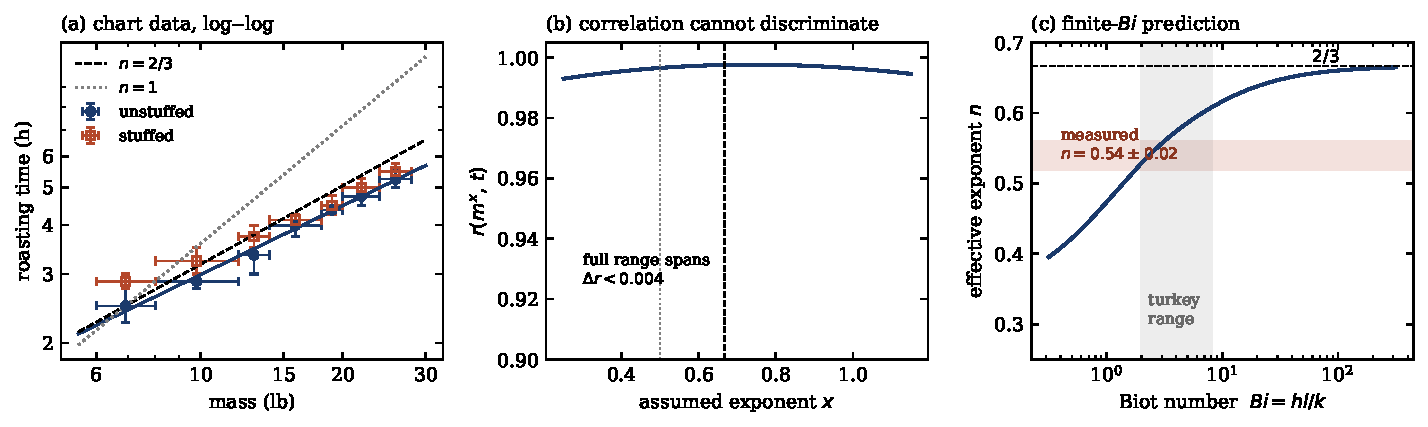
\includegraphics[width=\textwidth]{fig1.pdf}
\caption{(a) Chart data with fitted power law; the $n=1$ and $n=2/3$ lines
are anchored at the smallest bird. (b) Correlation coefficient
$r(m^{x},t)$ against assumed exponent $x$: the whole range spans less than
$0.004$, so $r$ cannot discriminate. (c) Effective exponent from
Eq.~\eqref{eq:neff} against Biot number, with the range spanned by
\SIrange{6}{28}{\pound} birds shaded and the measured value in red.}
\label{fig:main}
\end{figure}

Weighted log--log regression gives
\begin{align}
\text{unstuffed:}\quad & n = \num{0.61 \pm 0.05},\\
\text{stuffed:}\quad & n = \num{0.49 \pm 0.04},\\
\text{joint fit (common exponent):}\quad & n = \num{0.54 \pm 0.02},
\end{align}
the joint fit allowing separate prefactors, which differ by a factor
\num{1.08}. Referred to the unstuffed fit, the proportional law $n=1$ is
excluded at $7.5\sigma$; $n=2/3$ lies at $1.1\sigma$ and $n=1/2$ at
$2.0\sigma$. The fitted relation is
\begin{equation}
t\,[\mathrm{h}] \;=\; 0.78\;\bigl(m\,[\mathrm{lb}]\bigr)^{0.59},
\label{eq:fit}
\end{equation}
valid over \SIrange{6}{28}{\pound} at \SI{325}{\degreeFahrenheit}.

Three points deserve emphasis. First, the two columns do not return the
same exponent, which sets a floor on what these data can resolve: the
honest statement is $n \approx 0.55 \pm 0.05$, not a value to three
decimals. Second, that value is consistent with the finite-Biot prediction
of Section~\ref{sec:correct}, so no departure from diffusive physics need
be invoked. Third, a competing explanation exists and cannot be separated
here: a turkey is not self-similar, and large birds grow in length and
breadth more than in thickness, so the relevant half-thickness scales as
$l \propto m^{p}$ with $p < 1/3$, depressing $n$ by the same amount.
Distinguishing the two mechanisms requires thickness measurements, not
chart entries.

\section{A second data set: bread, and why it does not help}
\label{sec:bread}

Baking charts \cite{bread} are sometimes offered as an independent check.
They are not usable for this purpose, and the reason is instructive. In
the chart we examined, oven temperature falls as loaf mass rises
(\SI{523}{\kelvin} for small rolls, \SI{488}{\kelvin} for a \SI{1}{\kilo\gram}
boule): $\ln m$ and $\ln T$ have a sample correlation of $-0.75$. Mass and
temperature effects are therefore collinear and not separately
identifiable. A mass-only fit returns $n = 0.53$ with $R^{2}=0.89$; adding
a free temperature exponent raises $R^{2}$ to $0.99$ but returns an
exponent of $-8.8$ on $T$, which is physically meaningless and simply
absorbs the collinearity. The improvement is a property of the design
matrix, not evidence for a temperature correction.

Bread differs from poultry in other ways that matter: a loaf loses
\SIrange{15}{20}{\percent} of its mass to evaporation during baking, and its
doneness criterion involves crust formation rather than a core temperature
alone. We report the analysis only to caution against it.

\section{A corrected exercise}
\label{sec:exercise}

The pedagogical value of the problem survives if it is posed on real
numbers and with the modelling step made explicit. We suggest:

\begin{quote}
\itshape
A \SI{24}{\pound} turkey roasts in \SI{5.2}{\hour} at \SI{325}{\degreeFahrenheit}.
(a) Assuming the bird is geometrically similar and that heat transport is
diffusion-limited with an isothermal surface, estimate the time for a
\SI{10}{\pound} bird. (b) The published chart gives \SIrange{2.75}{3.0}{\hour}.
Your estimate is slightly high. Identify which assumption fails, and show
that relaxing it moves the prediction in the right direction.
\end{quote}

Part (a) gives $5.2\times(10/24)^{2/3} = \SI{2.9}{\hour}$, inside the
chart range. Part (b) is the point of the exercise: the isothermal-surface
assumption is $\Bi \to \infty$, whereas $\Bi \approx 3$ here, and
Eq.~\eqref{eq:neff} lowers the exponent towards the measured $0.55$.
Students end with a correct number, an explicit model, and a named
assumption to question --- rather than with eight hours and a turkey that
would be inedible.

\section{Conclusion}

The turkey problem is a good exercise built on bad data and an unstated
modelling step. Three conclusions follow.

Dimensional analysis does not select among power laws; the variable list
does. Enumerating admissible monomials over a list containing both
$\alpha$ and $k,\rho,c$, and both $m$ and $l$, produced sixteen formulae
that reduce to six, ten of them containing an absolute temperature that
the linearity of the heat equation forbids. Correctly posed, the problem
gives one group and two parameters, $\Fo = F(\Bi,\theta_{c})$.

Correlation coefficients cannot be used to choose an exponent. On these
data they vary by less than $0.004$ over $x\in[0.3,1.0]$ and peak at the
wrong value. Log--log regression with stated uncertainties is the minimum
acceptable tool.

The measured exponent, $n = \num{0.54 \pm 0.02}$, is below $2/3$ and far
from $1$. Both a finite Biot number and departure from geometric
similarity predict a deficit of the observed size, and chart data cannot
separate them. Resolving that is the natural experiment: instrument birds
of several masses with core probes, record thickness as well as mass, and
repeat at two oven temperatures so that $\theta_{c}$ is varied
independently.

\subsection*{Data and code availability}

All fits, the monomial reduction of Table~\ref{tab:collapse}, and
Fig.~\ref{fig:main} are reproducible from the scripts accompanying this
note, available at
\url{https://github.com/l0d0v1c/TurkeyDimensional}.
\emph{[Add repository DOI before submission.]}

\subsection*{Declaration of competing interest}

\emph{[If any software cited here is authored or distributed by the
authors, declare it explicitly in this section.]}

\begin{thebibliography}{99}

\bibitem{buckingham1914}
E.~Buckingham, On physically similar systems: illustrations of the use of
dimensional equations, \emph{Phys. Rev.} \textbf{4} (1914) 345--376.
\href{https://doi.org/10.1103/PhysRev.4.345}{doi:10.1103/PhysRev.4.345}.

\bibitem{barenblatt1996}
G.~I. Barenblatt, \emph{Scaling, Self-Similarity, and Intermediate
Asymptotics}, Cambridge University Press, 1996.

\bibitem{incropera}
T.~L. Bergman, A.~S. Lavine, F.~P. Incropera, D.~P. DeWitt,
\emph{Fundamentals of Heat and Mass Transfer}, 8th ed., Wiley, 2017,
ch.~5 (one-term approximations for transient conduction).

\bibitem{rossi2001}
L.~F. Rossi, Contemporary applications of mathematics, course notes,
University of Delaware, 2001.
\emph{[Replace with an archived or printed source; the original URL is
dead.]}

\bibitem{buffalo}
Dimensional analysis lecture notes, State University of New York at
Buffalo.
\emph{[Replace with an archived or printed source; the original URL is
dead.]}

\bibitem{usda}
U.S. Department of Agriculture, Food Safety and Inspection Service,
\emph{Safe Minimum Internal Temperature Chart}.
\emph{[Add current URL and access date.]}

\bibitem{chart}
Commercial poultry roasting chart, oven at \SI{325}{\degreeFahrenheit}.
\emph{[Add publisher, edition and access date; several independent charts
should be compared, since a single one is not an independent measurement.]}

\bibitem{bread}
Baking time chart for bread.
\emph{[Add publisher and access date.]}

\end{thebibliography}

% ---------------------------------------------------------------------
% For elsarticle, replace \title/\author/\maketitle above by:
%
% \begin{frontmatter}
% \title{The turkey problem revisited: what dimensional analysis can and
%        cannot decide}
% \author[a]{l0d0v1c}
% \author[a]{pseudoLucV7}
% \address[a]{\url{https://github.com/l0d0v1c/TurkeyDimensional}}
% \begin{abstract} ... \end{abstract}
% \begin{keyword} dimensional analysis \sep Biot number \sep scaling \end{keyword}
% \end{frontmatter}
% ---------------------------------------------------------------------

\end{document}
